\section{Tensor structured CC in the strong correlation limit
\label{sec:strong_correlation}}
\subsection{Introduction}
In this section we will discuss the behavior of tensor structured CC methods 
in the strong correlation regime, as well as some possible future lines of 
research. As was mentioned in Chapter~\ref{ch:introduction}, strong correlation 
presents a major challenge to current many-body methods. Standard 
coupled cluster methods perform poorly for strong correlation, unless allowed 
to break proper physical symmetries of the wavefunction or very high orders of 
excitation operators are taken into account. Both of the latter options are 
implausible in applications.

The simplest case when strong correlation arises in molecular systems is the 
dissociation of multielectron bonds and various transition state 
configurations. Model Hamiltonians are also a convenient benchmark for 
many-body methods in strong correlation. The eigenstates of the Hubbard 
Hamiltonian at half-filling are strongly correlated when the on-site repulsion 
is significantly higher than the kinetic energy, e.g. $\eta = U / t \gg 0$. We 
used these two settings to test the behavior of tensor structured coupled 
cluster methods.

\subsection{Rank restriction in TCC at strong correlation}
All coupled cluster calculations in this section used up to 2000 iterations and 
$10^{-8}$ convergence threshold. Other parameters were chosen in the same 
way as described in Sections~\ref{sec:thc_rccsd} and~\ref{sec:cpd_rccsd}. 

As a first test, we applied CPD-RCCSD to Hubbard models with $6$, $10$ and $14$ 
sites. 
%
\begin{figure}[ht!]
\centering
%\begin{subfigure}{0.75\textwidth}
%\centering
%\includegraphics[width=1\linewidth]
%{figures/tcc_strong_correlation/energy_vs_u_6_sites_cpd_rccsd}
%\caption{6 sites}
%\label{fig:energy_vs_u_6_sites_cpd_rccsd}
%\end{subfigure}
%\begin{subfigure}{0.75\textwidth}
%\centering
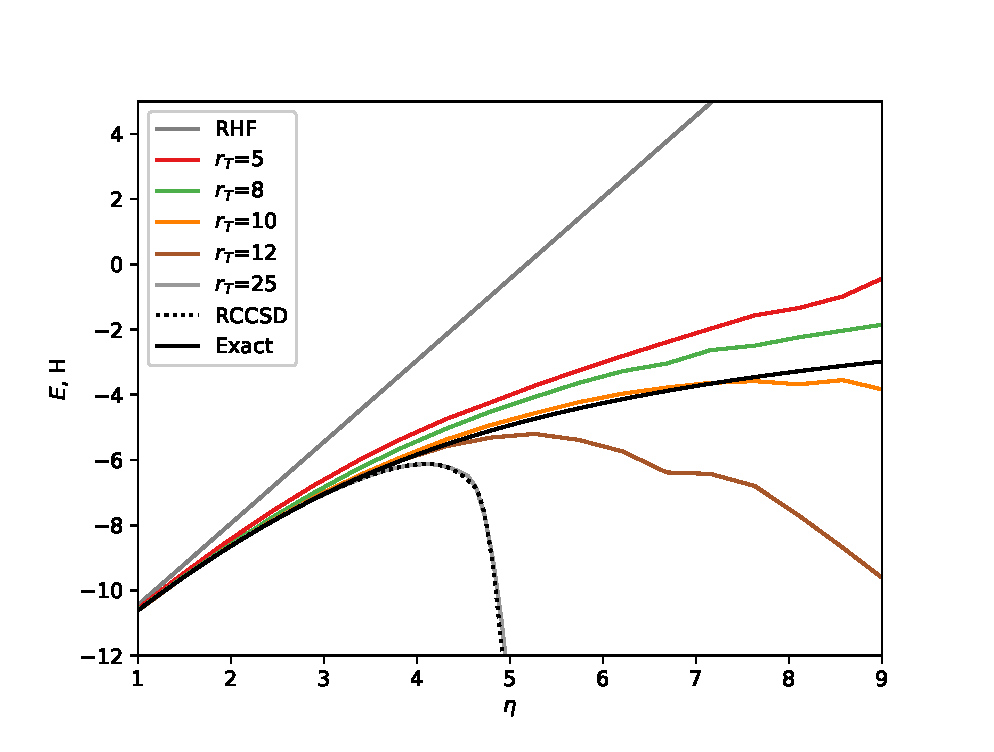
\includegraphics[width=\columnwidth]
{figures/tcc_strong_correlation/energy_vs_u_10_sites_cpd_rccsd}
%\caption{10 sites}
%\label{fig:energy_vs_u_10_sites_cpd_rccsd}
%\end{subfigure}
\caption{Energy behavior for different ranks of CP decomposition of amplitudes. 
Hubbard model at half-filling, 10 sites}
\label{fig:energy_vs_u_cpd}
\end{figure}
%
Figure~\ref{fig:energy_vs_u_cpd} shows the dependence of the total energy 
on the interaction strength $\eta$. As expected, conventional RCCSD provides 
a good description of Hubbard rings at low $\eta$, and systematically 
overestimates the energy as the system becomes strongly correlated. CPD-RCCSD, 
however, demonstrates a surprising effect. If one chooses the approximation to 
the doubles amplitudes to be the low 
rank, the incorrect behavior of the original RCCSD method may be fixed. As the 
rank is increased, the solutions of CPD-RCCSD gradually change behavior between 
the Hartree-Fock (no correlation) and conventional RCCSD 
(overestimation of correlation energy), as can be seen on 
Figure~\ref{fig:energy_vs_u_cpd}. This situation, however, is not 
specific to CPD-RCCSD, and is also observed with THC-RCCSD (see 
Figure~\ref{fig:energy_vs_u_thc}).
%
\begin{figure}[ht!]
\centering
%\begin{subfigure}{0.75\textwidth}
%\centering
%\includegraphics[width=1\linewidth]
%{figures/tcc_strong_correlation/energy_vs_u_6_sites_thc_rccsd}
%\caption{6 sites}
%\label{fig:energy_vs_u_6_sites_thc_rccsd}
%\end{subfigure}
%\begin{subfigure}{0.75\textwidth}
%\centering
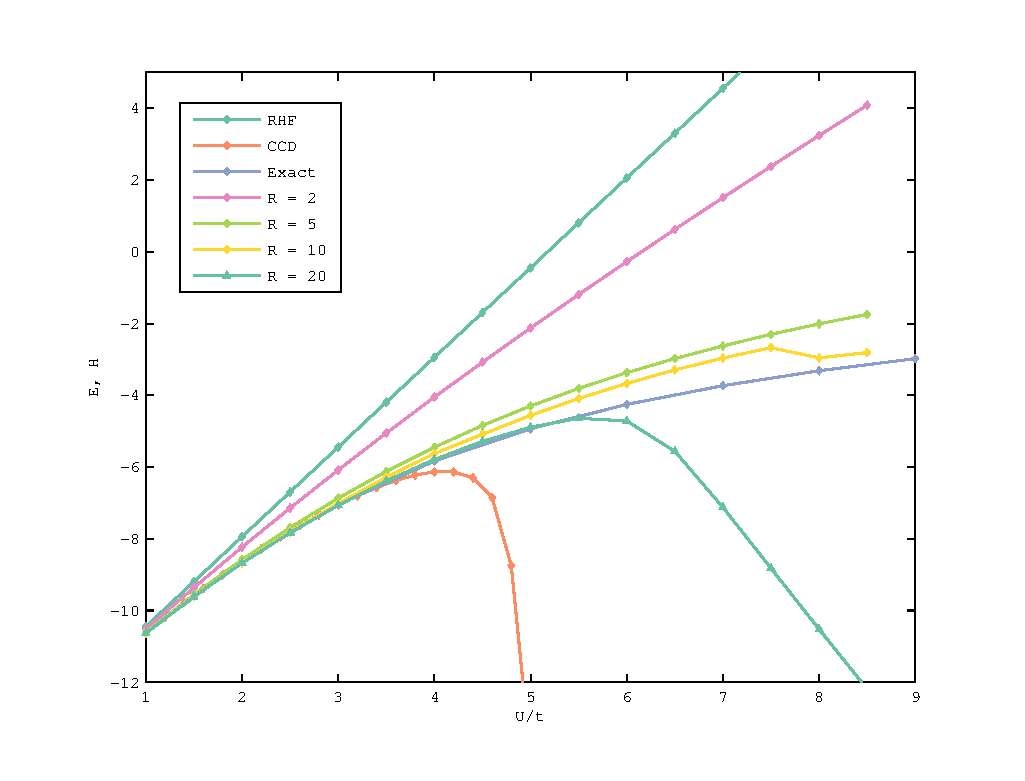
\includegraphics[width=\columnwidth]
{figures/tcc_strong_correlation/energy_vs_u_10_sites_thc_rccsd}
%\caption{10 sites}
%\label{fig:energy_vs_u_10_sites_thc_rccsd}
%\end{subfigure}
\caption{Energy behavior for different ranks of THC decomposition of 
amplitudes. Hubbard model at half-filling, 10 sites}
\label{fig:energy_vs_u_thc}
\end{figure}
%
The difference in the case of THC-RCCSD is that the overcorrelation happens at 
slightly larger ranks (compare, for example, $r_{T} = 5$ and $r_{T} = 10$ 
between Figures~\ref{fig:energy_vs_u_cpd} and \ref{fig:energy_vs_u_thc}). Both 
methods, however, reproduce standard RCCSD when sufficiently large ranks of the 
decompositions are chosen, as one may expect.

The results observed with the Hubbard Hamiltonian do not change qualitatively 
in the case of molecular systems. Figure~\ref{fig:energy_vs_d_cc-pvdz} 
demonstrates the effect of rank restriction in CPD-RCCSD for the calculation of 
the dissociation curve of nitrogen. With rank equal 4, the solution has the 
correct behavior at the dissociation limit, while for larger ranks CPD-RCCSD 
approximates standard RCCSD. The rank restricted solutions, however, miss a 
fair amount of weak correlation energy, which plays a major role in molecular 
systems (near the equilibrium exact and 
CPD-RCCSD curves are far apart). Having seen the behavior of rank restricted 
approximate coupled cluster for a wide range of systems, we would like to 
provide an interpretation of the observed effect.
%
\begin{figure}[!ht]
\centering
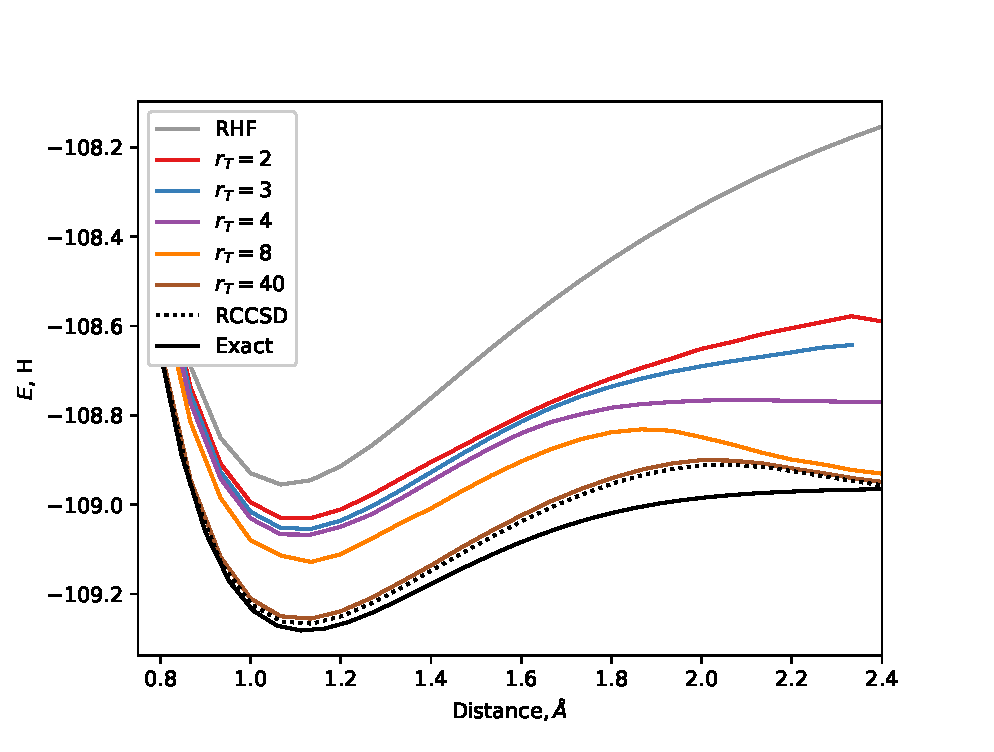
\includegraphics[width=\columnwidth]
{figures/tcc_strong_correlation/energy_vs_d_cc-pvdz}
\caption{Energy behavior for different ranks of CP decomposition of 
amplitudes. Dissociation of nitrogen, cc-pVDZ}
\label{fig:energy_vs_d_cc-pvdz}
\end{figure}
%

\subsection{Tentative explanation}
Let us offer a tentative explanation of the observed effect based on additional 
parameters of the rank-restricted solutions. As was noted before, at strong 
correlation several configurations become degenerate and this degeneracy 
is caused by physical symmetries encoded in the 
Hamiltonian.\cite{scuseria2011projected,jimenez2012projected} Some of the 
entries of excitation operators, which correspond to degenerate configurations, 
have to get larger and larger values. We argue that this imbalance, namely a 
significantly higher importance of a small subset of amplitudes over the rest of 
them, is what makes residual equations in coupled cluster an ill-posed problem. 
This may be paralleled to solving an overdetermined nonlinear system.

Degroote~\emph{et al.}~\cite{degroote2016polynomial} demonstrated
that in the strong correlation regime cluster amplitude tensors may factorize, 
e.g. that the effective number of parameters in cluster amplitudes is lower. 
The later is the idea behind their polynomial similarity transformation theory, 
which uses general polynomial series instead of an exponent to parameterize 
the wavefunction. The non-exponential similarity transformation leads to a 
different set of residual equations, where dominant amplitudes have larger 
contributions to the residual. The amplitudes in these CC-like methods do not 
grow to large values, in contrast with traditional coupled cluster.
A similar situation is observed with rank-restricted solutions in our approach.

%
\begin{figure}[ht]
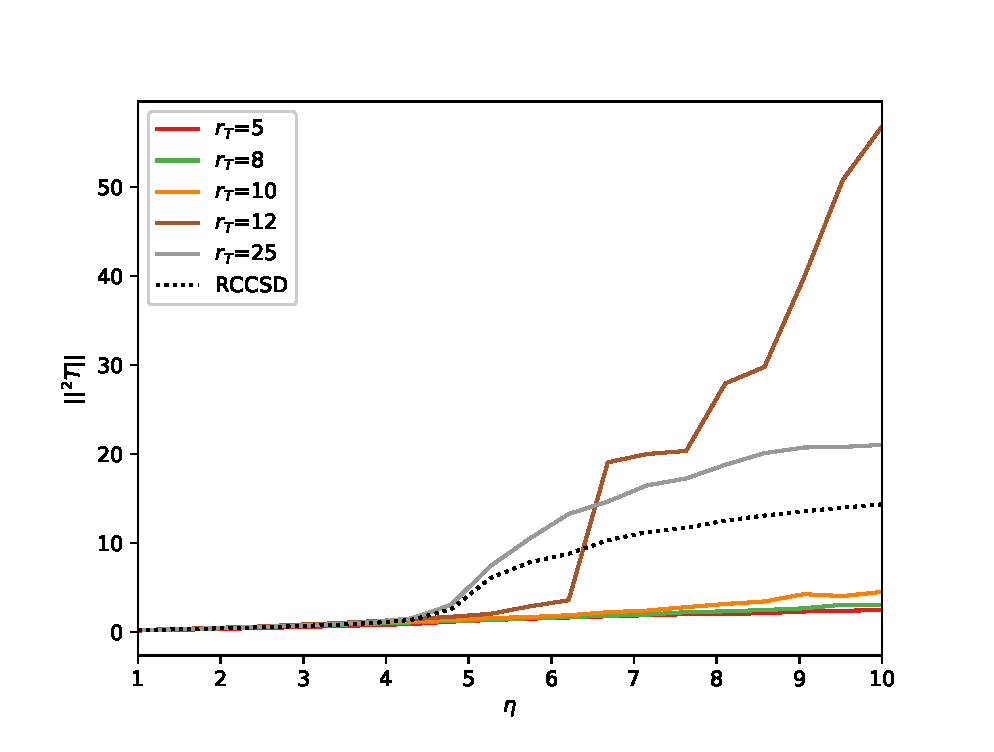
\includegraphics[width=\columnwidth]
{figures/tcc_strong_correlation/t2_norms_vs_u_10_sites_cpd_rccsd}
\caption{Frobenius norm of ~ ${}^2T$ amplitudes for different ranks $r_{T}$ in 
CPD-RCCSD 
calculations. Hubbard model at half-filling, 10 sites.
\label{fig:t2_norms_vs_u_10_sites_cpd_rccsd}}
\end{figure}
%
In Figure~\ref{fig:t2_norms_vs_u_10_sites_cpd_rccsd} the dependence of the norm 
of the ${}^2T$ amplitudes as a function of rank and on-site repulsion is shown. 
As the graph illustrates, the norm of the doubles amplitudes in the physically 
proper-behaving low rank solutions is lower than the norm of ${}^2T$ amplitudes 
in conventional RCCSD. In contrast, as the ranks grow and CPD-RCCSD starts 
to overcorrelate, there is a sharp increase in the amplitude norm to values 
even higher than the standard RCCSD would yield. For example, the solution with 
$r_{T} = 12$, which significantly overcorrelates at $\eta > 6$ (see 
Figure~\ref{fig:energy_vs_u_cpd}, yellow line) also has large 
norm of ${}^2T$ amplitudes starting at the same values of $\eta$ 
(Figure~\ref{fig:t2_norms_vs_u_10_sites_cpd_rccsd}, yellow line). 

Moreover, the low-rank solutions in tensor structured CC 
do not satisfy the standard residual equations in analogy to the CC-like 
method of Degroote~\emph{et al.} we mentioned.
Figure~\ref{fig:r2_norms_vs_u_10_sites_cpd_rccsd} demonstrates the 
dependence of the residual norm on the correlation strength parameter $\eta$ 
for different ranks. The physically well behaving cluster amplitudes deviate 
from being the solutions of the residual equations as $\eta$ increases.
The individual factors in the decomposition of amplitudes, however, \emph{do} 
satisfy their own ALS-like equations (see Chapter~\ref{ch:tcc}). The CC 
residuals are large for low-rank solutions and sharply drop as 
CPD-RCCSD amplitudes approach regular RCCSD amplitudes as one may 
expect (compare $r_{T} = 8$ 
and $r_{T} = 25$ in 
Figures~\ref{fig:energy_vs_u_thc},~\ref{fig:t2_norms_vs_u_10_sites_cpd_rccsd} 
and~\ref{fig:r2_norms_vs_u_10_sites_cpd_rccsd}). 
%
\begin{figure}[ht]
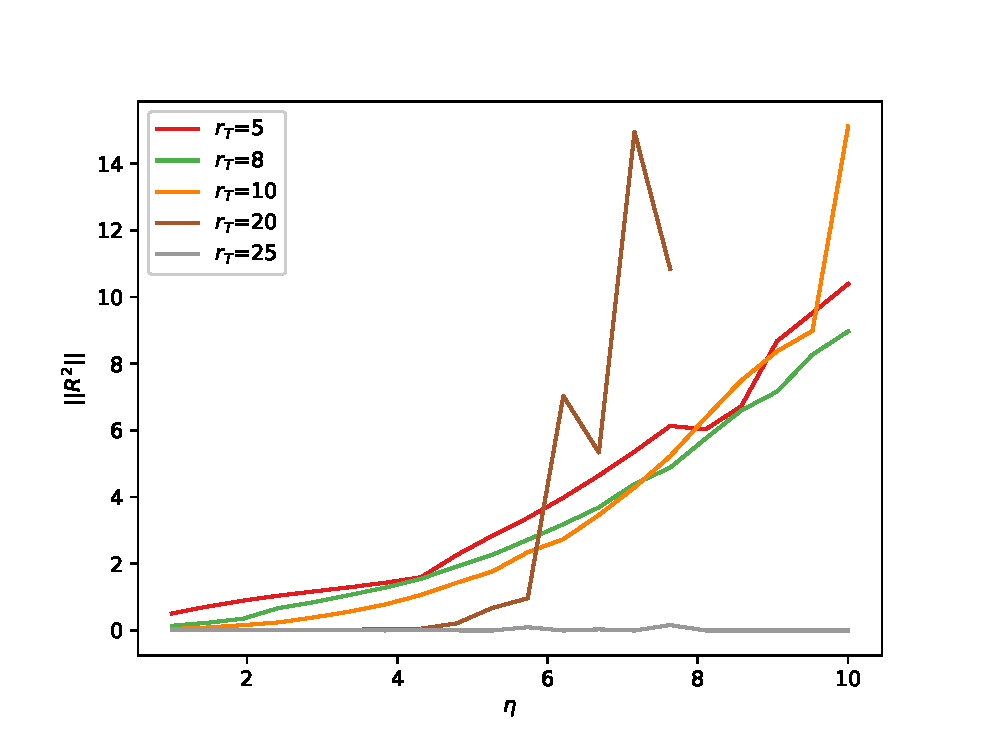
\includegraphics[width=\columnwidth]
{figures/tcc_strong_correlation/r2_norms_vs_u_10_sites_cpd_rccsd}
\caption{Frobenius norm of ~${}^2T$ residuals for different ranks $r_{T}$ in 
CPD-RCCSD 
calculations. Hubbard model at half-filling, 10 sites}
\label{fig:r2_norms_vs_u_10_sites_cpd_rccsd}
\end{figure}
%
To summarize our observations, rank restriction of the 
amplitudes seems to be a way to regularize conventional CC equations 
in strong correlation regime. We would like to point out that similar 
regularization schemes (called "dropout regularization") are ubiquitous in 
machine learning literature.~\cite{srivastava2014dropout, wan2013regularization} 
This raises a question whether other regularization techniques, like 
standard $l_{2}$-norm regularization,\cite{tikhonov1963solution} can be applied 
in the coupled cluster method.

Let us mention last that the idea of Degroote~\emph{et 
al.}~\cite{degroote2016polynomial} was further developed in our group in a 
series of publications~\cite{degroote2016polynomial, gomez2017attenuated, 
qiu2017projected2, hermes2017combining}. In these works different 
similarity transformations were developed for specific model Hamiltonians. While 
being highly efficient both at strong and weak correlation regimes, these
CC-like methods use different ansatze for each symmetry responsible for 
the onset of strong correlation. The search for a universal approach for
strongly correlated systems thus still continues.

\subsection{Conclusions}
The strong correlation regime poses a hard problem for most many-body methods. 
Coupled cluster methods, while being very effective for weakly correlated 
systems, fail when strong correlation dominates. Recently a series of 
promising CC-like theories was developed in our 
group.\cite{degroote2016polynomial, gomez2017attenuated, 
qiu2017projected2, hermes2017combining} 
The problem of these theories, however, is that the explicit form of equations 
depends on the symmetry of the Hamiltonian responsible for the onset of strong 
correlation, and the idea is hard to generalize for arbitrary Hamiltonians. On 
the other hand, rank restriction in tensor structured CC provides a alternative 
way to regularize the solutions of standard coupled cluster at strong 
correlation, independently of the form of the Hamiltonian. More research is 
needed to make this approach practically applicable, but we believe the idea 
may be interesting in future method development.